% Autor: Daniel Tatzel

\section{Privater Ordner}

Der Private Ordner kann über den Link \url{ebenezer-kunatse.net/private/} über das Menü aufgerufen werden, wenn er angemeldet ist, dies geschieht über den Menü-Punkt "`Privater Ordner"'. Es werden folgende Funktionen Angeboten:

% \bigskip

% \textbf{Funktionen:}

\begin{itemize}
 \item Die Buttons a. und b. blenden die Bereiche 1. und 2. ein und aus
 \item Im Bereich 1. kann durch Eingabe eines Passwortes und durch Absenden das Passwort für den Zugangsschutz ändern.
 \item Im Bereich 2. kann durch drücken des Buttons "`Browse"'eine Datei auf dem Computer ausgewählt werden. Durch drücken des "`Submit"' Buttons wird die Datei auf den Server geladen und ist in Bereich 3. sichtbar.
 \item In Bereich 3. ist eine Auflistung aller vorhandenen Dateien mit Namen (d) und Größe (e). Die Anzahl der anzuzeigenden Dateien (f) kann zwischen 10, 25, 50 und 100 variiert werden. Über die Seitenauswahl (g) kann zwischen den einzelnen Ergebnisseiten gewechselt werden. Eine Datei kann über den Button "`Löschen"' (c) gelöscht werden.
\end{itemize}


\begin{figure}[!htbp]
 \centering
 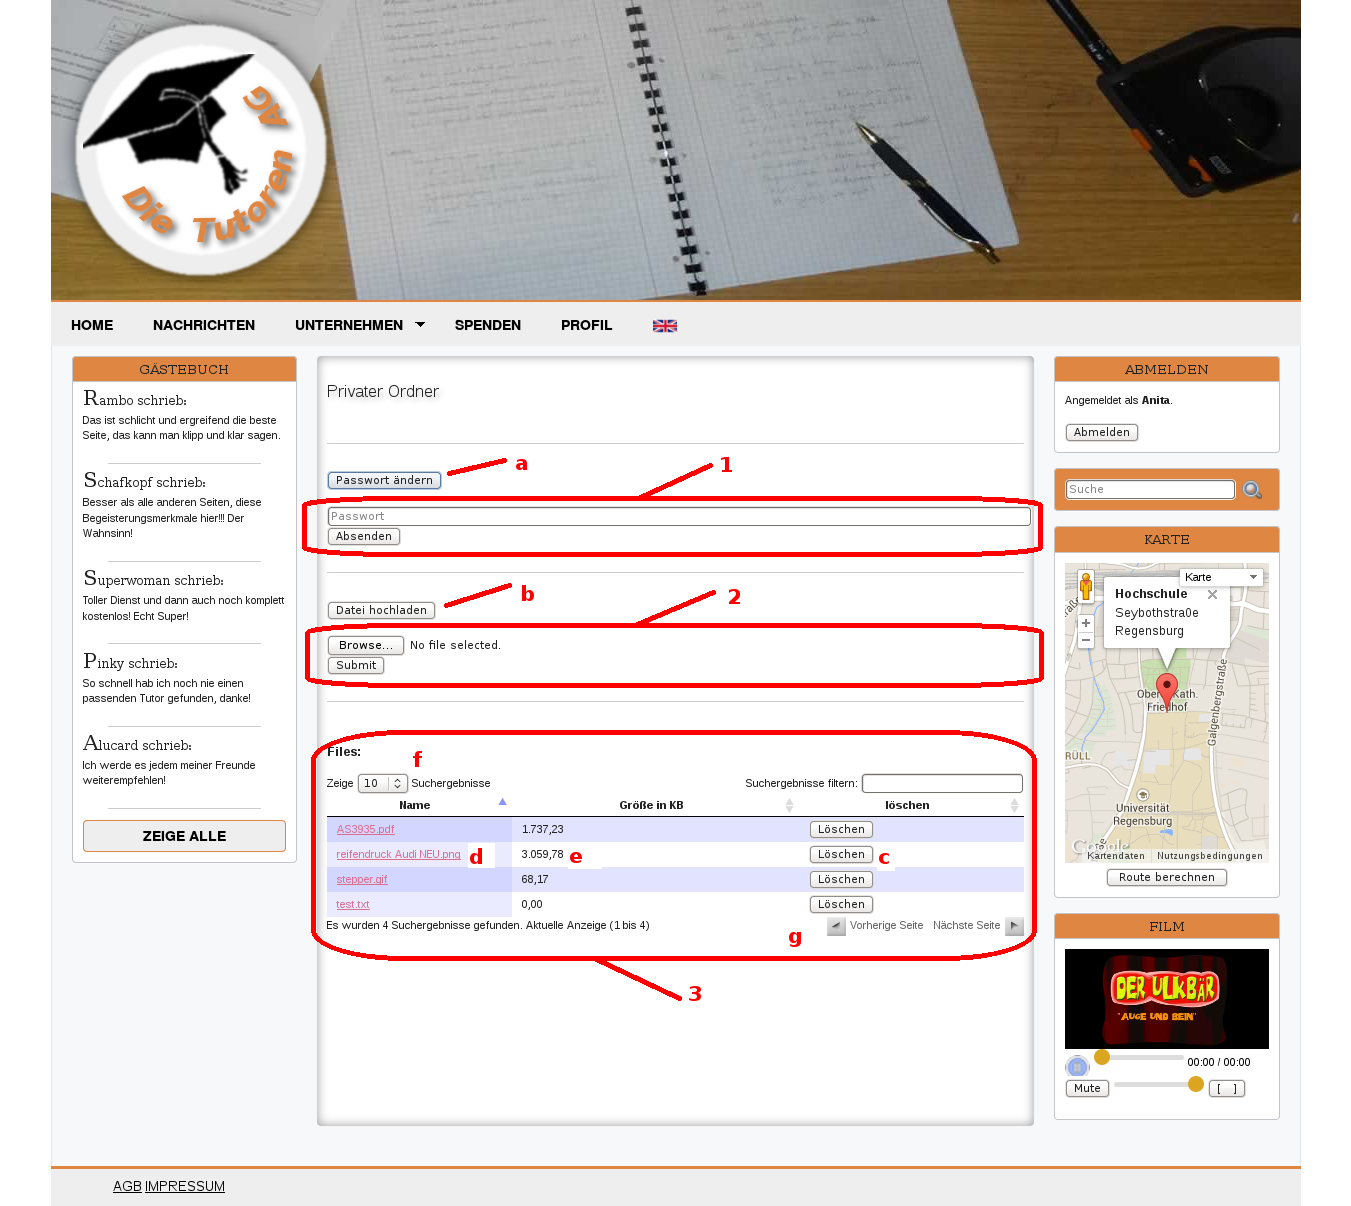
\includegraphics[width=1\textwidth]{../Screenshots/private/Privater_Ordner_passwd_upload}
 \label{fig:privatedir}
 \caption{Die Oberfläche des Privater Ordners}
\end{figure}

